
%----------------------------------------------------------------------------------------
%	PACKAGES AND OTHER DOCUMENT CONFIGURATIONS
%----------------------------------------------------------------------------------------

\documentclass[12pt]{article}
\usepackage[english]{babel}
\usepackage{amsmath}
\usepackage{graphicx}
\usepackage{float}
\usepackage[colorlinks = true,
linkcolor = blue,
urlcolor  = blue,
citecolor = blue,
anchorcolor = blue]{hyperref}
\usepackage{blindtext}
\usepackage{listings}
\usepackage{color}
\definecolor{light-gray}{gray}{0.95}
\lstset{
	numbers=left,
	breaklines=true,
	backgroundcolor=\color{light-gray},
	tabsize=2,
	basicstyle=\ttfamily,
}


\begin{document}
	
	\begin{titlepage}
		
		\newcommand{\HRule}{\rule{\linewidth}{0.5mm}} 
		
		\center % Center everything on the page
		
		%----------------------------------------------------------------------------------------
		%	HEADING SECTIONS
		%----------------------------------------------------------------------------------------
		\textsc{\Large MSc Project: Mobile Hairdresser Application}\\[5 cm] 

		
		
		
\includegraphics[scale=0.05]{images/logo.png}\\[1 cm]
				
		

		
		
		\textsc{\LARGE Joshua Robertson} \\[6 cm]
		
		

		
		
		%----------------------------------------------------------------------------------------
		%	TITLE SECTION
		%----------------------------------------------------------------------------------------
		
		
		
		%----------------------------------------------------------------------------------------
		%	AUTHOR SECTION
		%----------------------------------------------------------------------------------------
		
		
		\begin{center}
			
			\textsc\emph{{“A dissertation submitted to the University of Bristol in accordance with the requirements of the degree of Master of Science by advanced study in Computer Science in the Faculty of Engineering."}} \\[1.2 cm]
			
			School of Computer Science, Electrical and Electronic Engineering, and Engineering Maths (SCEEM) \\[1 cm]
			
			
			
		\end{center}
		
		
		
		
		\vfill % Fill the rest of the page with whitespace
		
	\end{titlepage}
	
	\section{Introduction}
	Plan - 
	1) Covid has caused an increase in homeworking
	2) People want greater access to remote services
	3) People also want quick access to products
	2 reasons for application is that people want fast and easy access to services, and it is expected now with companies i.e. amazon now offering same day delivery. and also peoples views around covid
	
	There is little dispute that the recent COVID-19 pandemic has had a significant impact on our daily lives. Along with having a devestating both on a societal and individual level, it has brought with it a shift in perceptions around leaving the home. Subsequently, this has led to a desire for homeworking and easier access to remote services, with employers . Even with a reduction in COVID cases following a wave of vaccinations, it is likely that home working will continue to a greater extent than was seen previously, with home workers showing an increase in job satisfaction \cite{flexjobs, 2019}, \cite{CNBC, 2020}, productivity, mental health \cite(flexjobs, 2020) and even making more money (ADD CITE). 
	Although there already exists several apps that allow for home bookings, none follow the "uber" model, of allowing for immediate booking and delivery of home haircuts. This app therefore will facilitate this, along with aiming to explore any other market gaps through early research.
	
	
	New Product Development refers to the entirety of processes leading to bringing a product to market and encompasses several steps as seen in figure \ref{fig:npd} below.
	\newline
	
	\begin{figure}[H]
		\centering
		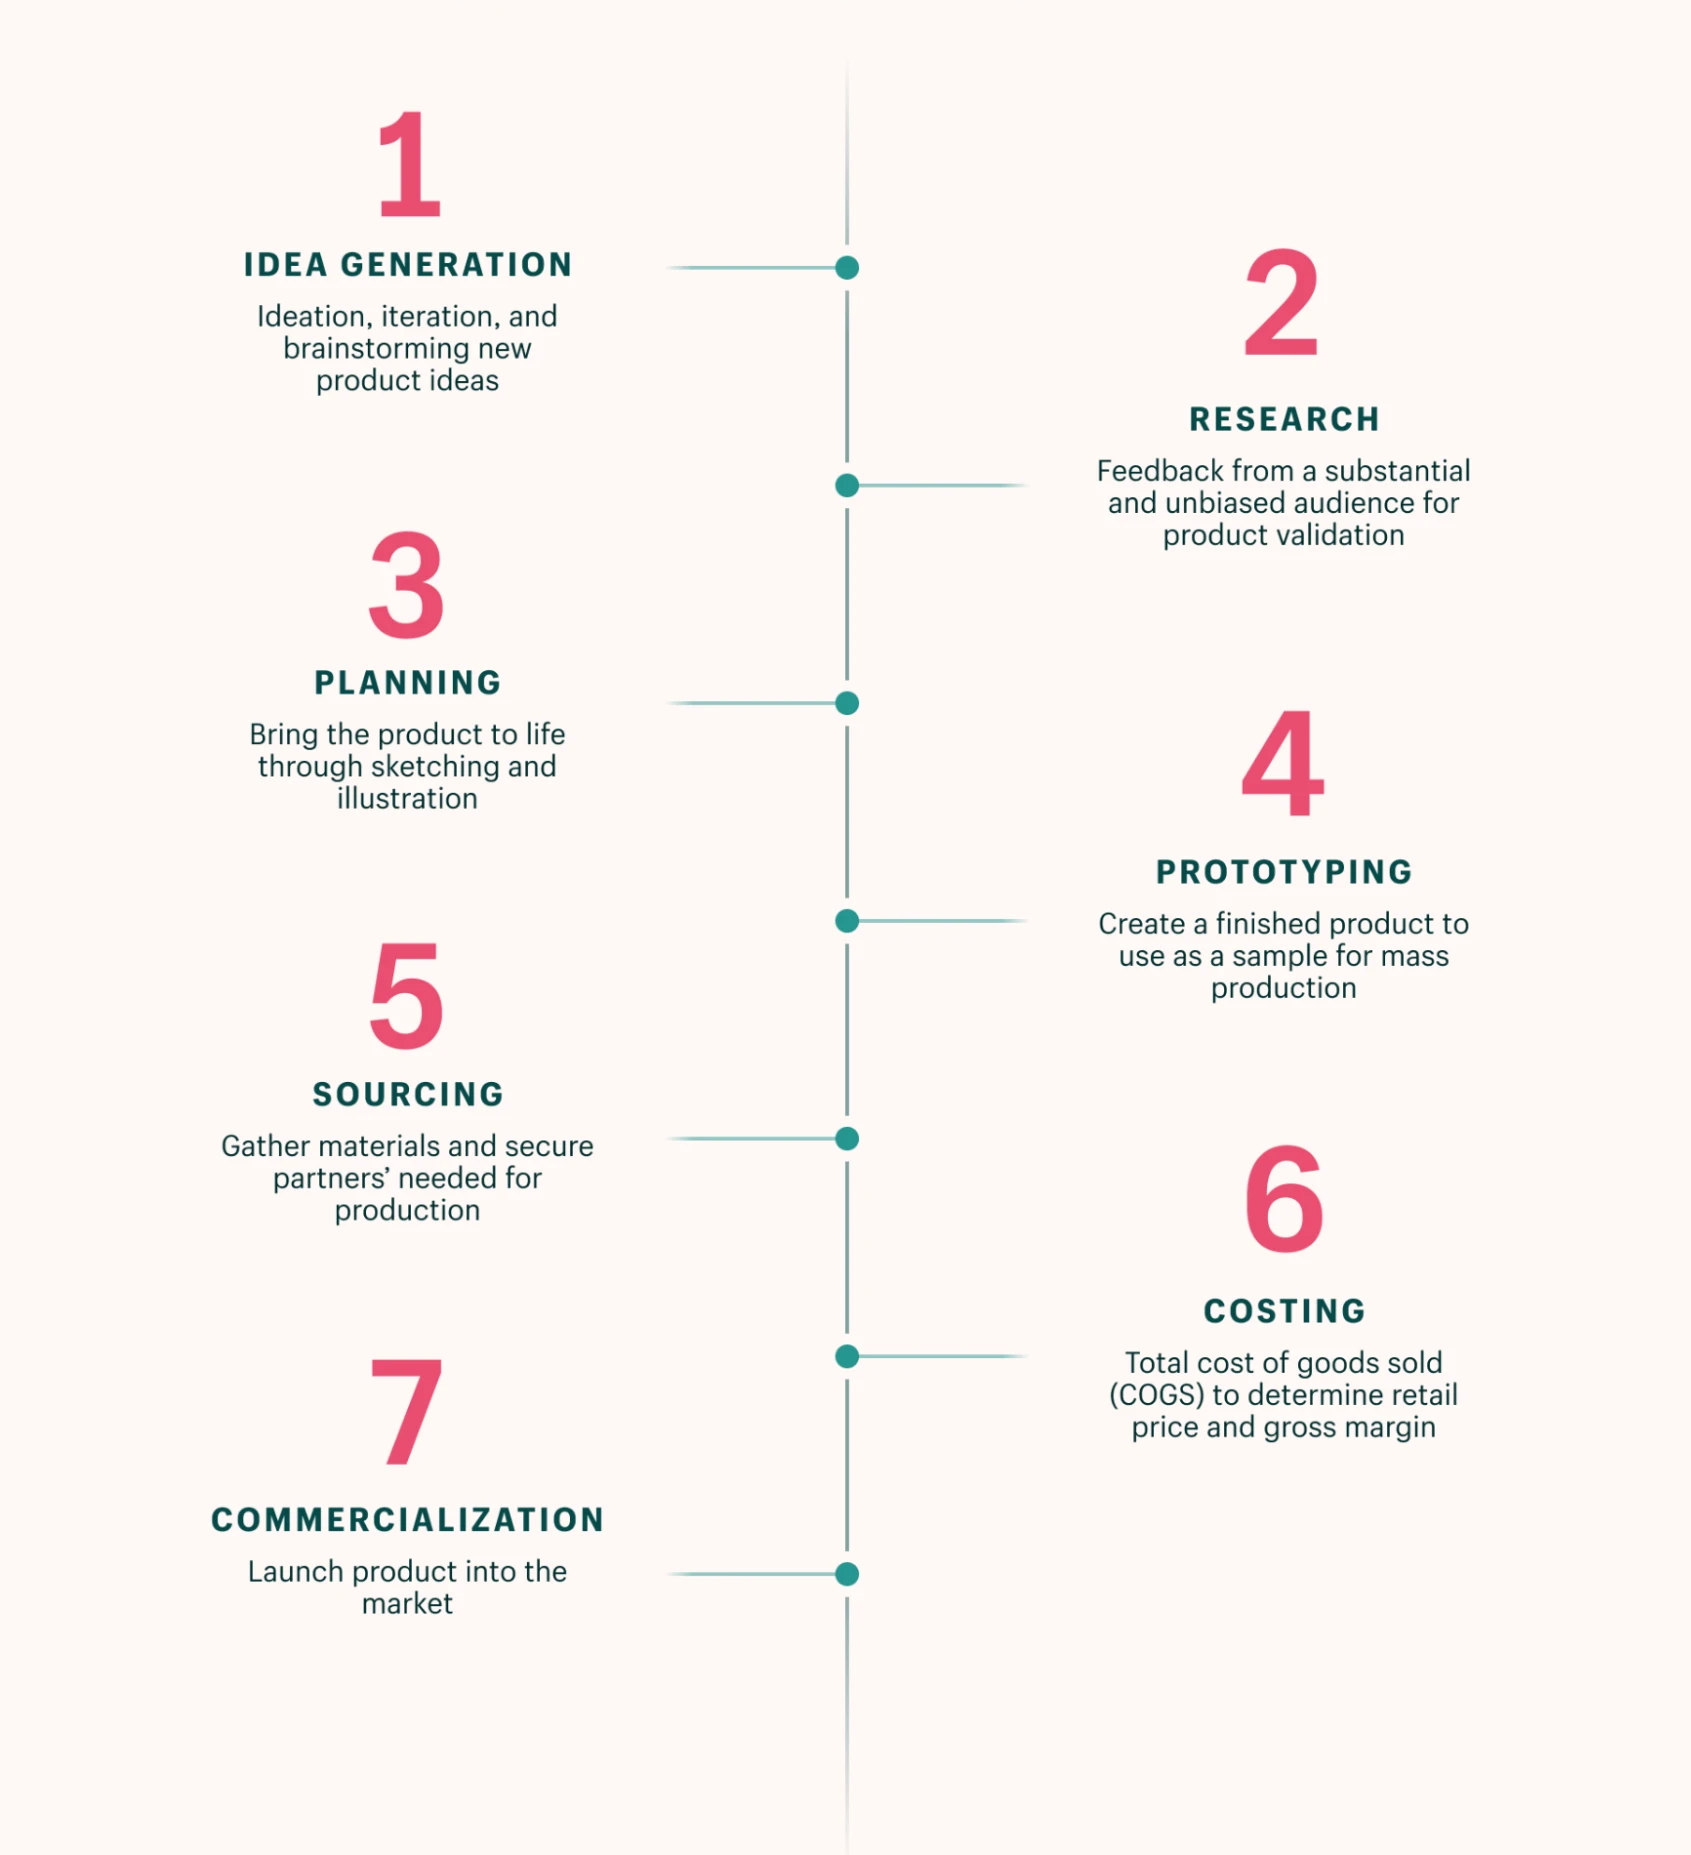
\includegraphics[scale=0.15]{images/npd.png}
		\caption{The 7 Steps of New Product Development}
		\label{fig:npd} \cite{shopify}
	\end{figure}
	
	
	\subsection{Ideation and Concept}
	\blindtext
	
	\subsection{Market Analysis}
	In order to gauge whether there is a market for the proposed analysis, a survey was carried out in which users were asked about whether they could see themselves using the application features, among other things.
	 
	\subsubsection{Existing Applications}
	As previously discusses there exists a variety of similar applications, for which the most prominent will be discussed below, along with
	
	\subsection{Deciding on a Platform}
	\subsubsection{Mobile vs Desktop}
	
	\subsubsection{Frontend: Android vs iOS}
	An important consideration when creating a mobile application is deciding on which platform to choose. The two largest mobile providers currently are android and apple (iOS). Historically, iOS has dominated the market share, with a 42.02\% market share in January 2011 compared to Androids 12.42\% (figure \ref{fig:ios-android}). Despite this, in recent years android OS has become more popular, even holding a greater share several times over the last few years and currently trails by only around 2\%.
	
	\begin{figure}[H]
		\centering
		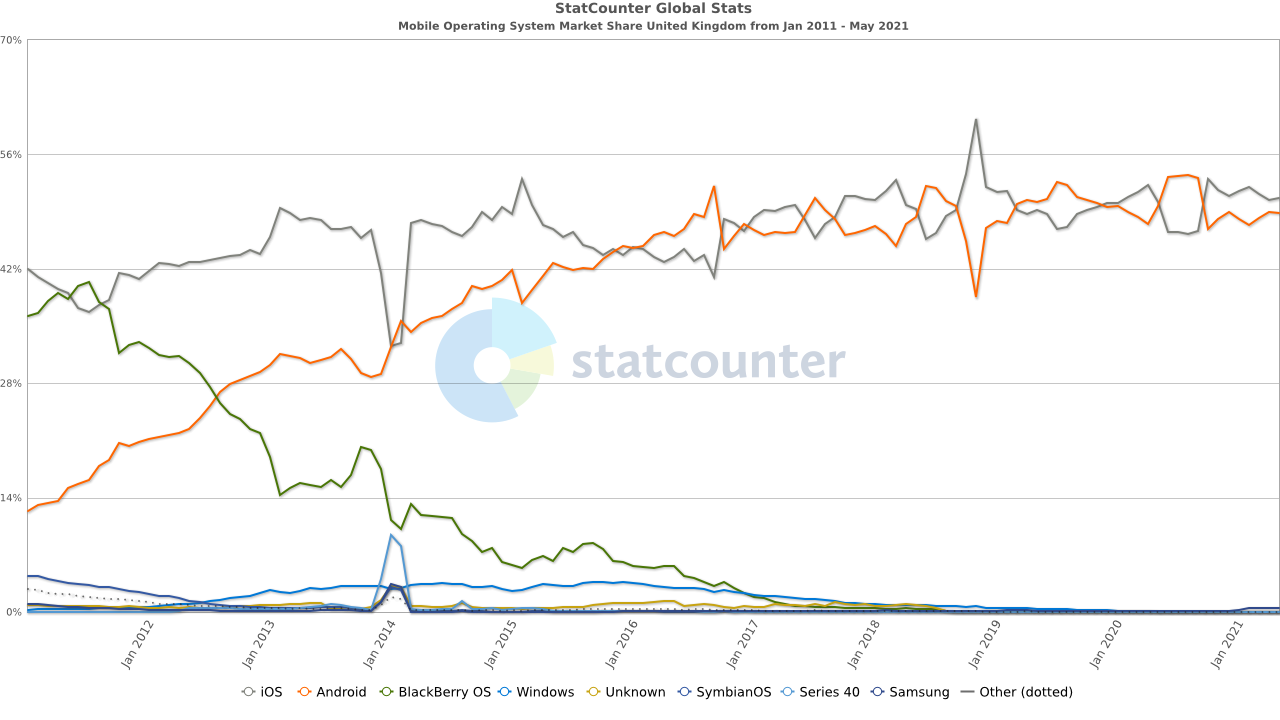
\includegraphics[scale=0.4]{images/ios-android.png}
		\caption{iOS vs Android Market Share Over The Last 10 Years}
		\label{fig:ios-android}
		\cite{stat-counter-21}
	\end{figure}
	
	With this change has brought with it a push towards frameworks that allow for development across multiple platforms, such as React Native (https://reactnative.dev/) and Flutter (flutter.dev/). For this reason, it was decided that a cross platform would be used, which is further discussed below.
	
	\subsection{Frontend: Programming Language}
	
	\subsection{Backend: SQL vs noSQL database}
	Initially a relational database model was created, which can be seen below (ADD DATABASE). This was later changed to use Google Firestore (\cite{firestore}), a noSQL database that relies on  nested 'documents' within 'collections'. This was chosen for several reasons. Firstly, as the chosen language 'Dart' is run by Google, using firestore allows for greater integration and congruence with the platform and APIs. Firestore also allows for rapid scalability, along with using Googles excellent cloud platform.
	
	Another important feature of noSQL databases is the ability to easily modify the internal data in response to changing business requirements, in an interative way that allows fordo you use relationship data in firebase stackoverflow modification throughout the application lifestyle and therefore easy scaling.
	Finally, the current model requires that each seperate barbers will need similar, although different data. For example, alough two barbers will likely share the product 'haircut', the description of each is likely to be entirely different making a normal SQL database difficult to implement.
	
	
	
	\subsubsection{The Target User}
	
	\subsubsection{Programming Language}
	When deciding on the programming software, several metrics were taken into consideration, including cross-platform functionality, speed, speed of development and performance. For this reason, Dart and the corresponding Flutter software development kit (SDK) were chosen for the primary software. Flutter is a cross-platform development kit, meaning that it will natively run on both iOS and android applications created by Google \cite{flutter}. Dart is compiled ahead-of-time into native ARM code giving better performance compared to other similar development kits, such as React Native and the user interface  is implemented within a fast, low-level C++ library giving great speed to the application. Dart has also seen a large increase in usage within recent years, jumping up 532\% from 2018 to 2019 \cite{Github, 2018} meaning that there is now an extensible list of third-party plugins available and a large community.
	

	\subsection{User Personas}
	The creation of user personas representing fictitious, archetypal users is an essential part of application development \cite{Grudin and Pruitt, 2002} and allows a deep understanding of the target user to be sought and implemented within the features and design of the application \cite{Long, 2009}. There are, however, some shortcomings to qualitative persona generation, such as validity concerns and user bias \cite{Chapman and Milham, 2007} and although they are addressed by other methods, such as data-driven personas \cite{Mcginn and Kotamraju, 2008}, there require a broad user base and therefore we have decided to stick with qualitative methods, which allow for enough brevity and depth for the scope of the project.
	
	Here 3 user personas were created, which are discussed in detail below.
	\begin{itemize}
		\item Persona 1: 
		
		Name: Sarah Johnson
		
		Profile: 
		\begin{figure}[H]

			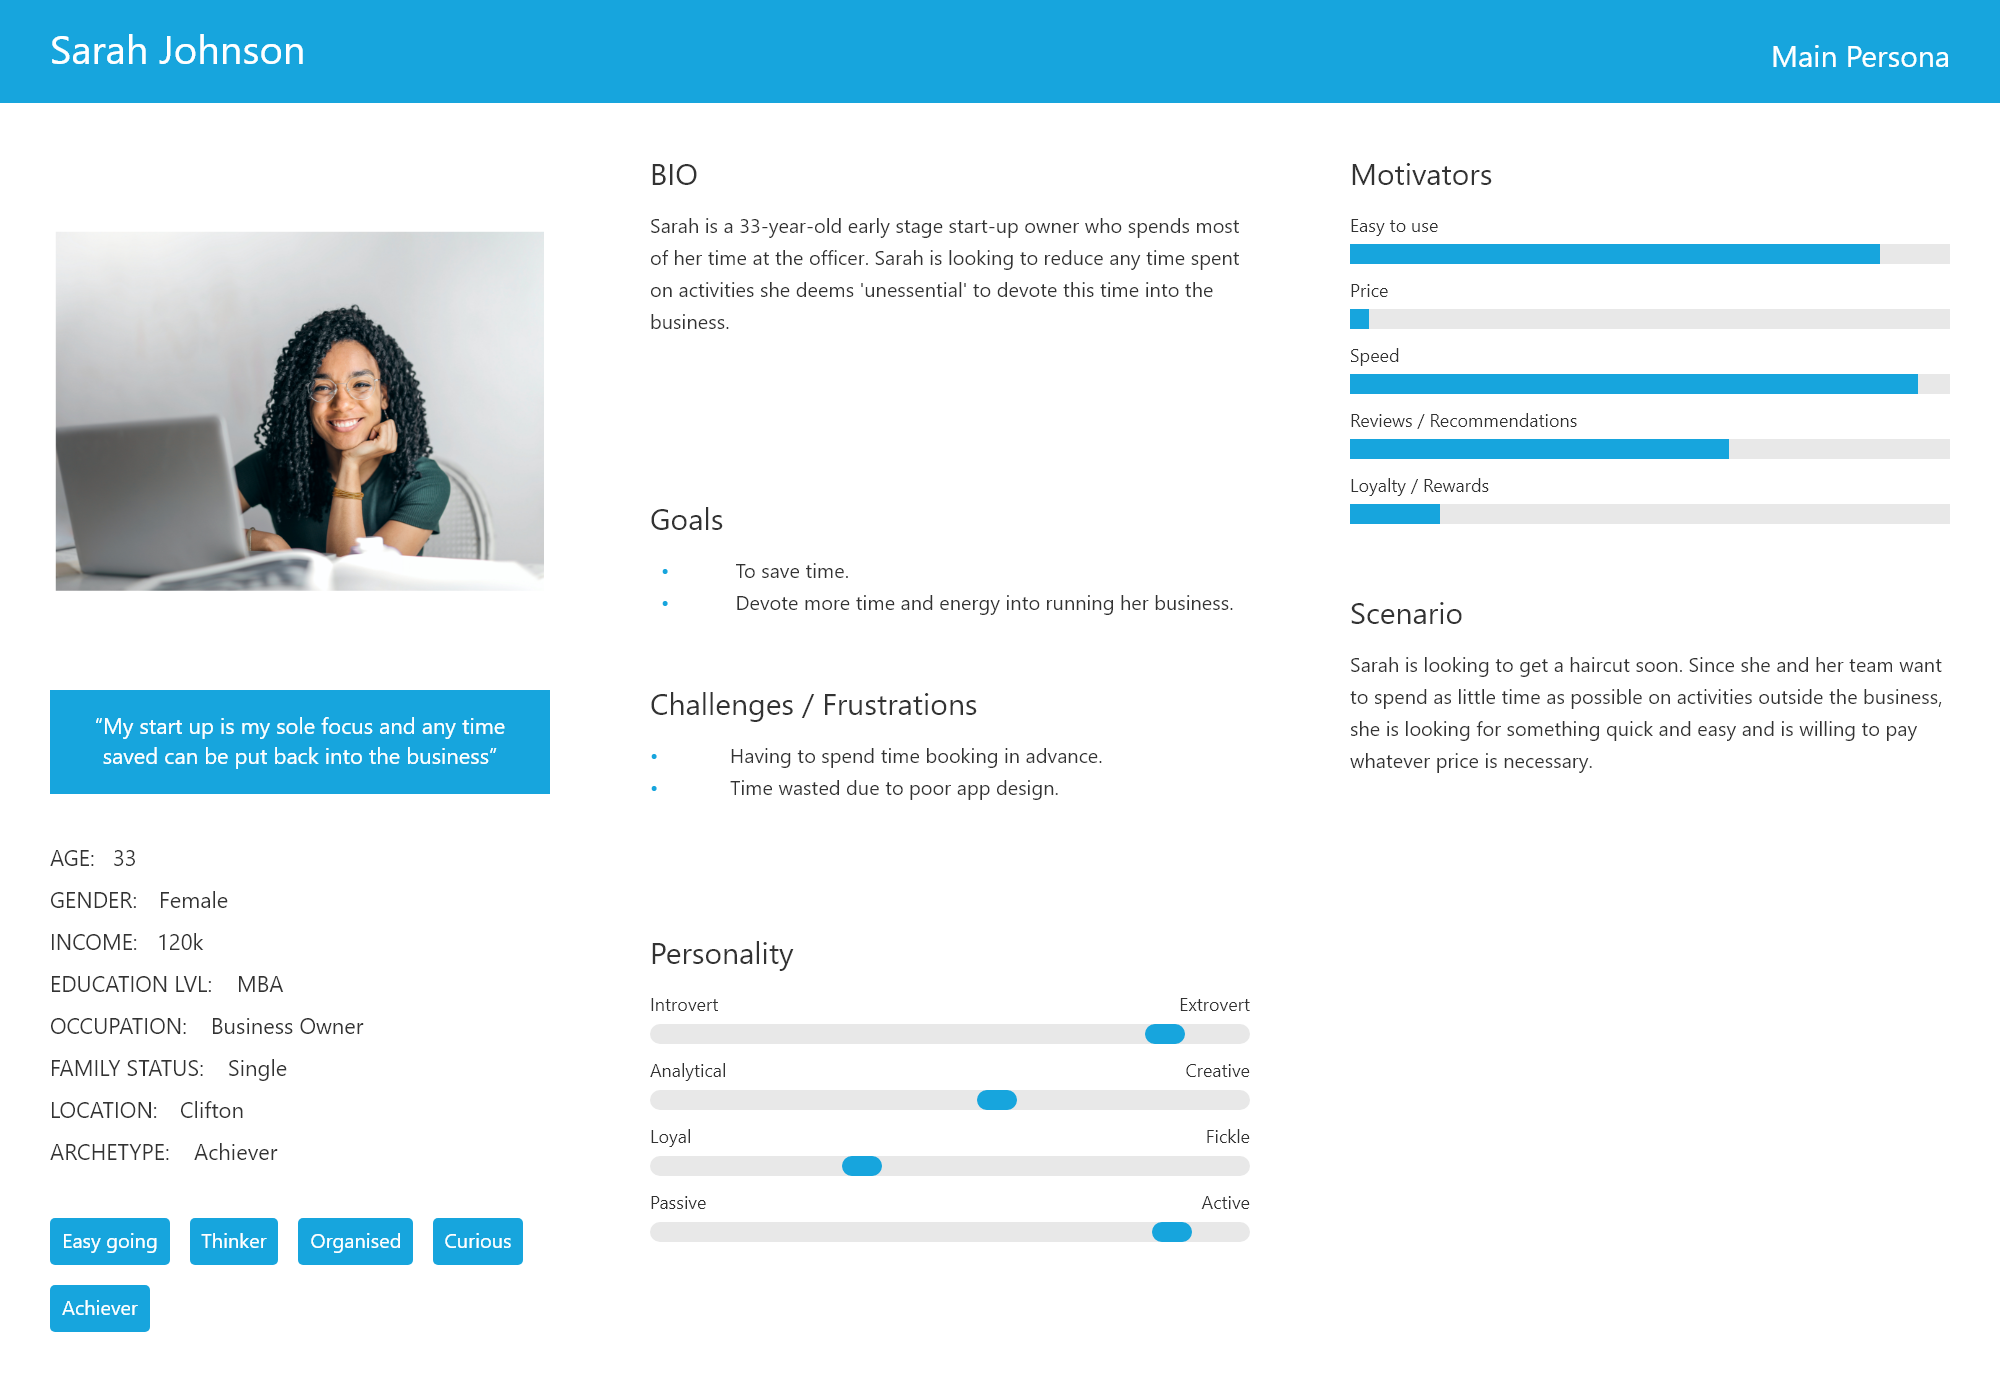
\includegraphics[scale=0.2]{images/persona_1.png}
			\caption{Persona 1}
			\label{fig:persona_1}
		\end{figure}
		
		\item Persona 2:
		
		Name:  Claire Sheppard
		
		
		Profile: 
		\begin{figure}[H]
			
			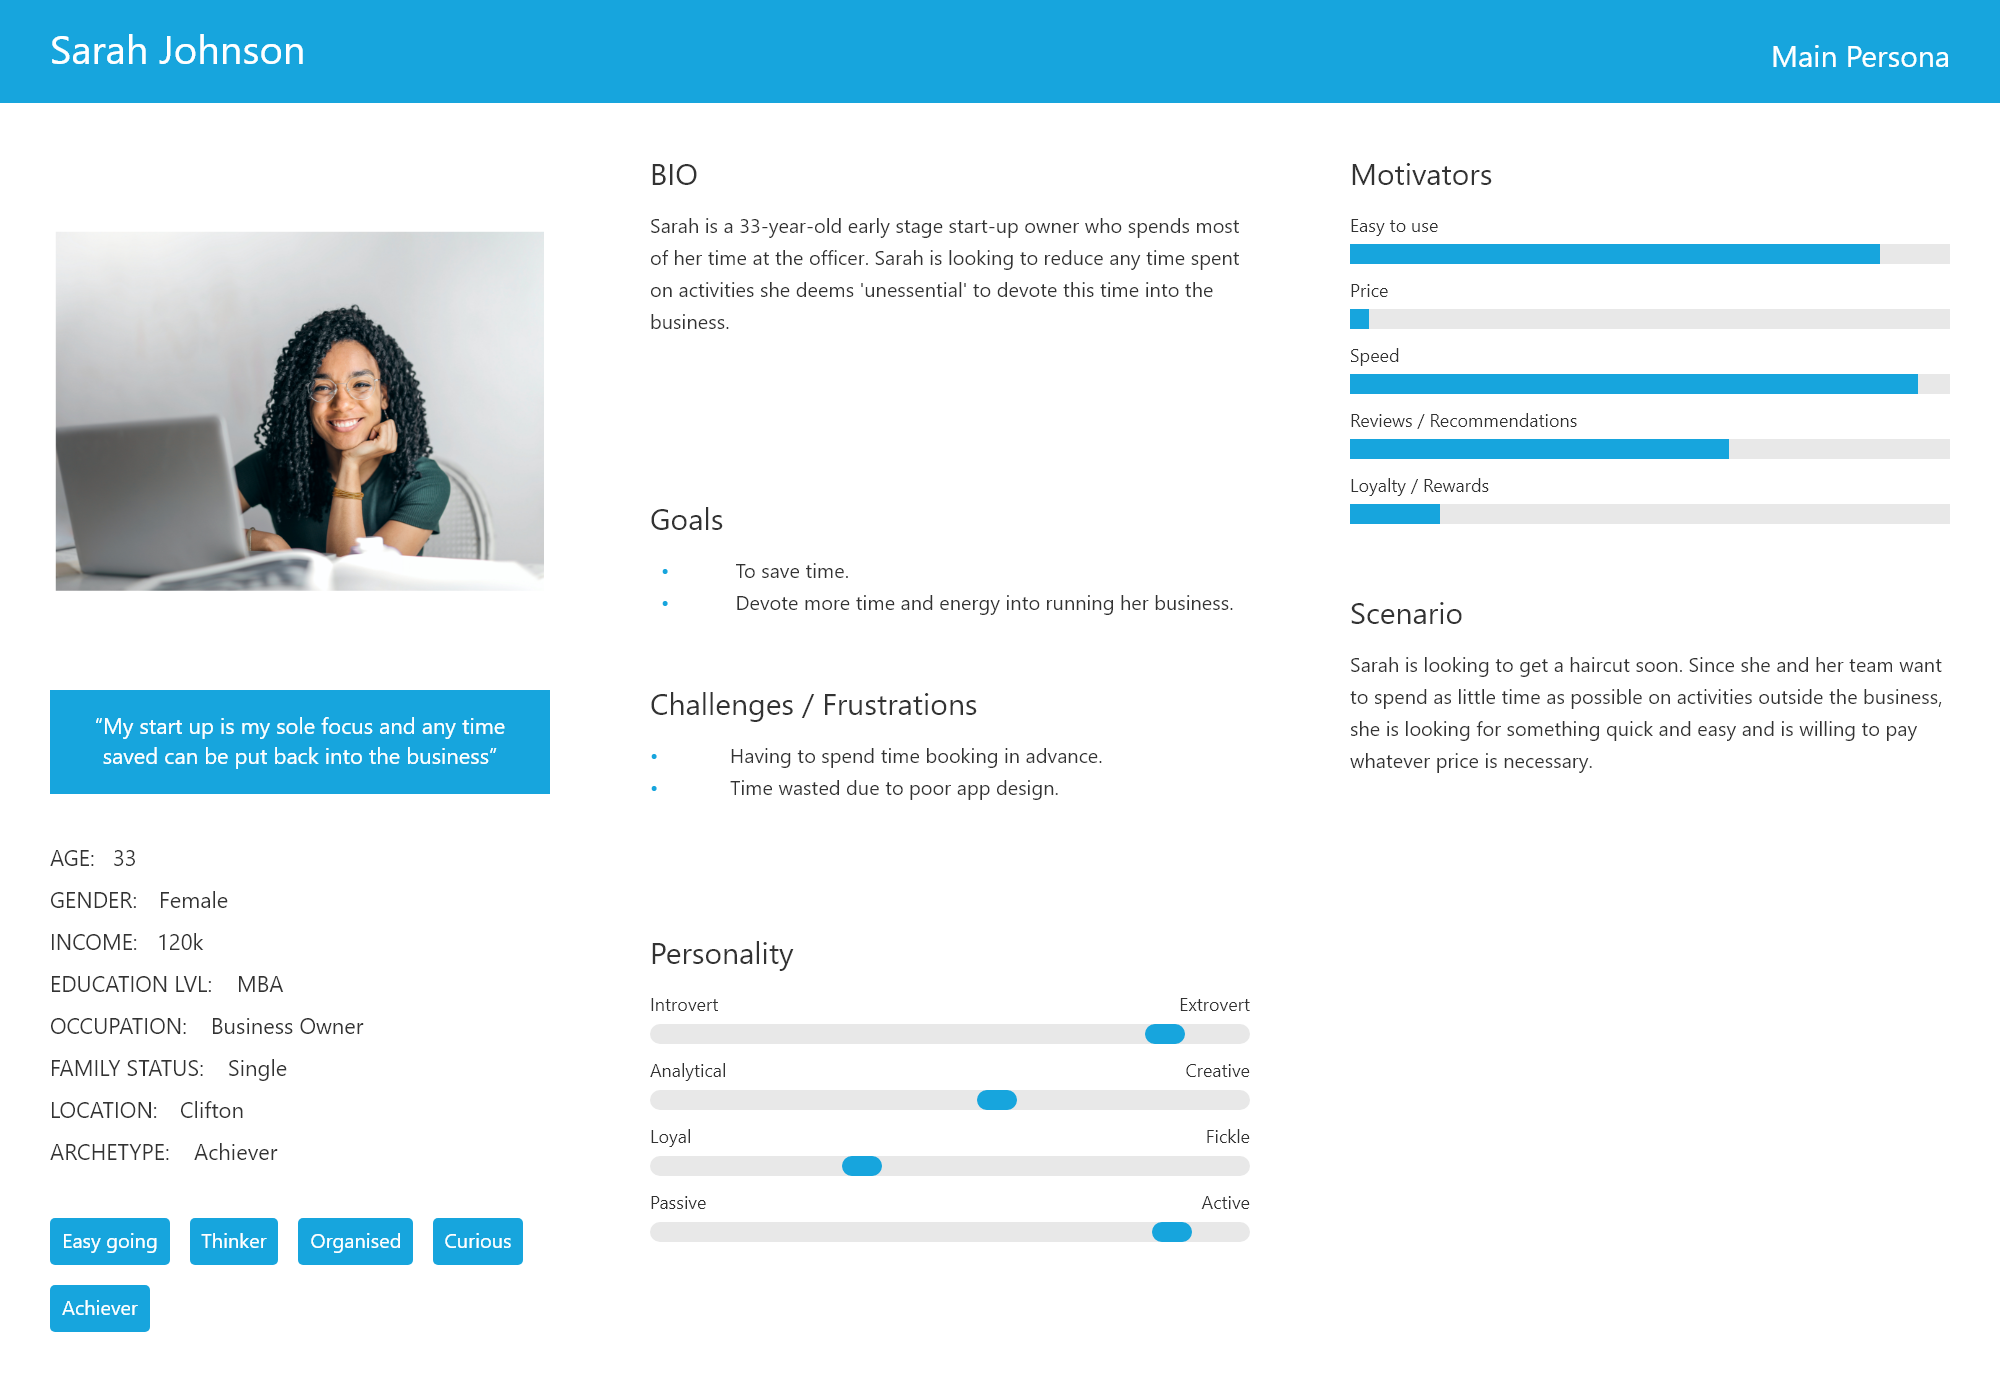
\includegraphics[scale=0.2]{images/persona_1.png}
			\caption{Persona 2}
			\label{fig:persona_2}
		\end{figure}
		
		\item Persona 3:
		
		Name: Emma Bradford
		
		Profile: 
		\begin{figure}[H]
			
			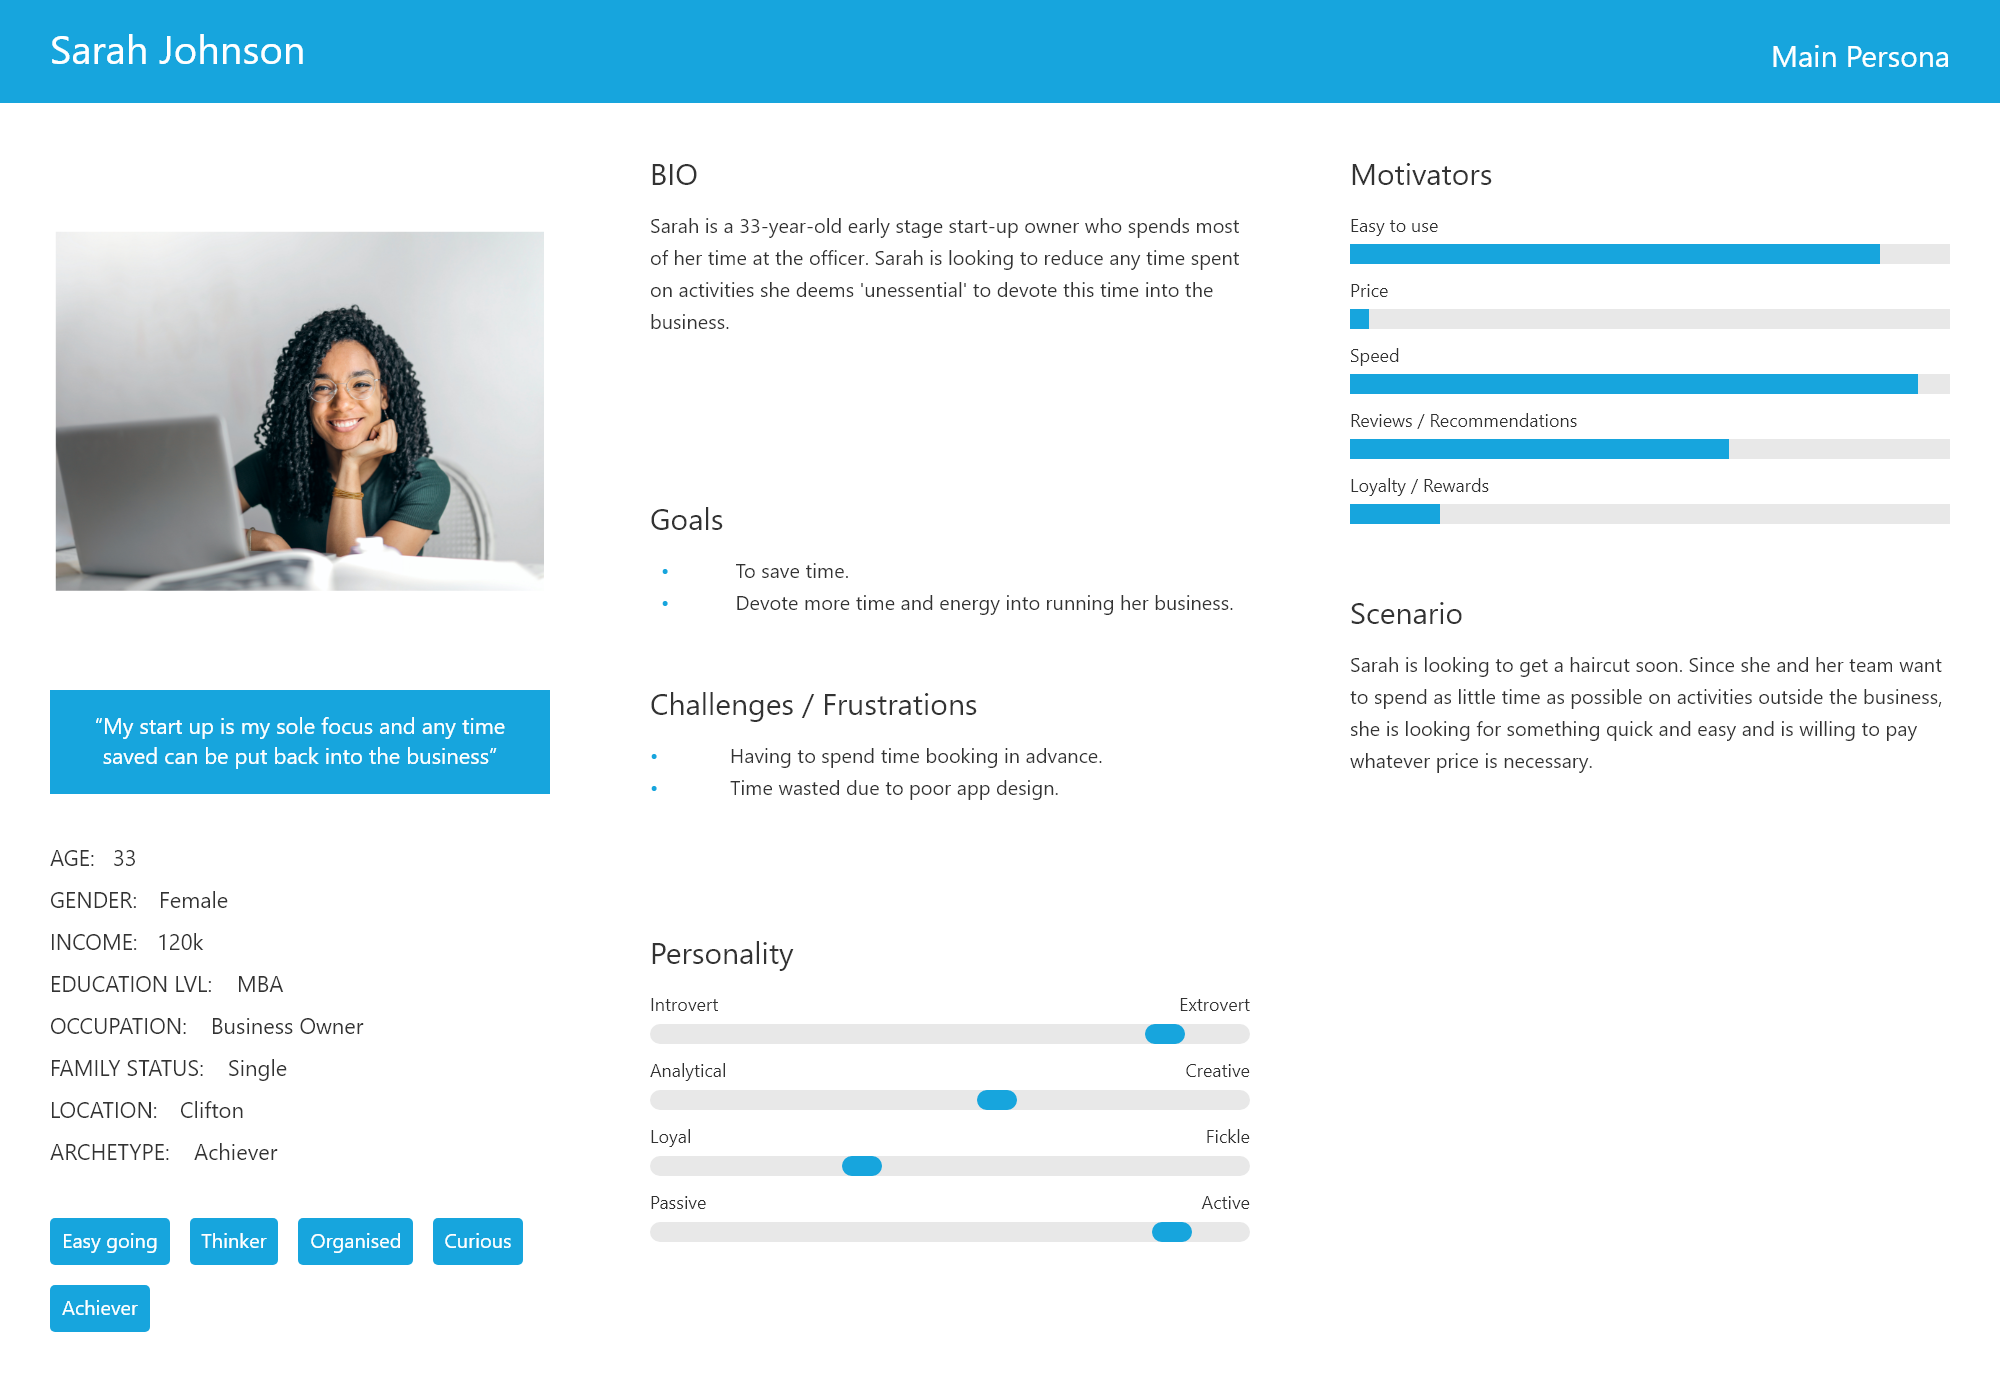
\includegraphics[scale=0.2]{images/persona_1.png}
			\caption{Persona 3}
			\label{fig:persona_3}
		\end{figure}
	
		\item Persona 4:
		
		Name:  Claire Sheppard
		
		
		Profile: 
		\begin{figure}[H]
			
			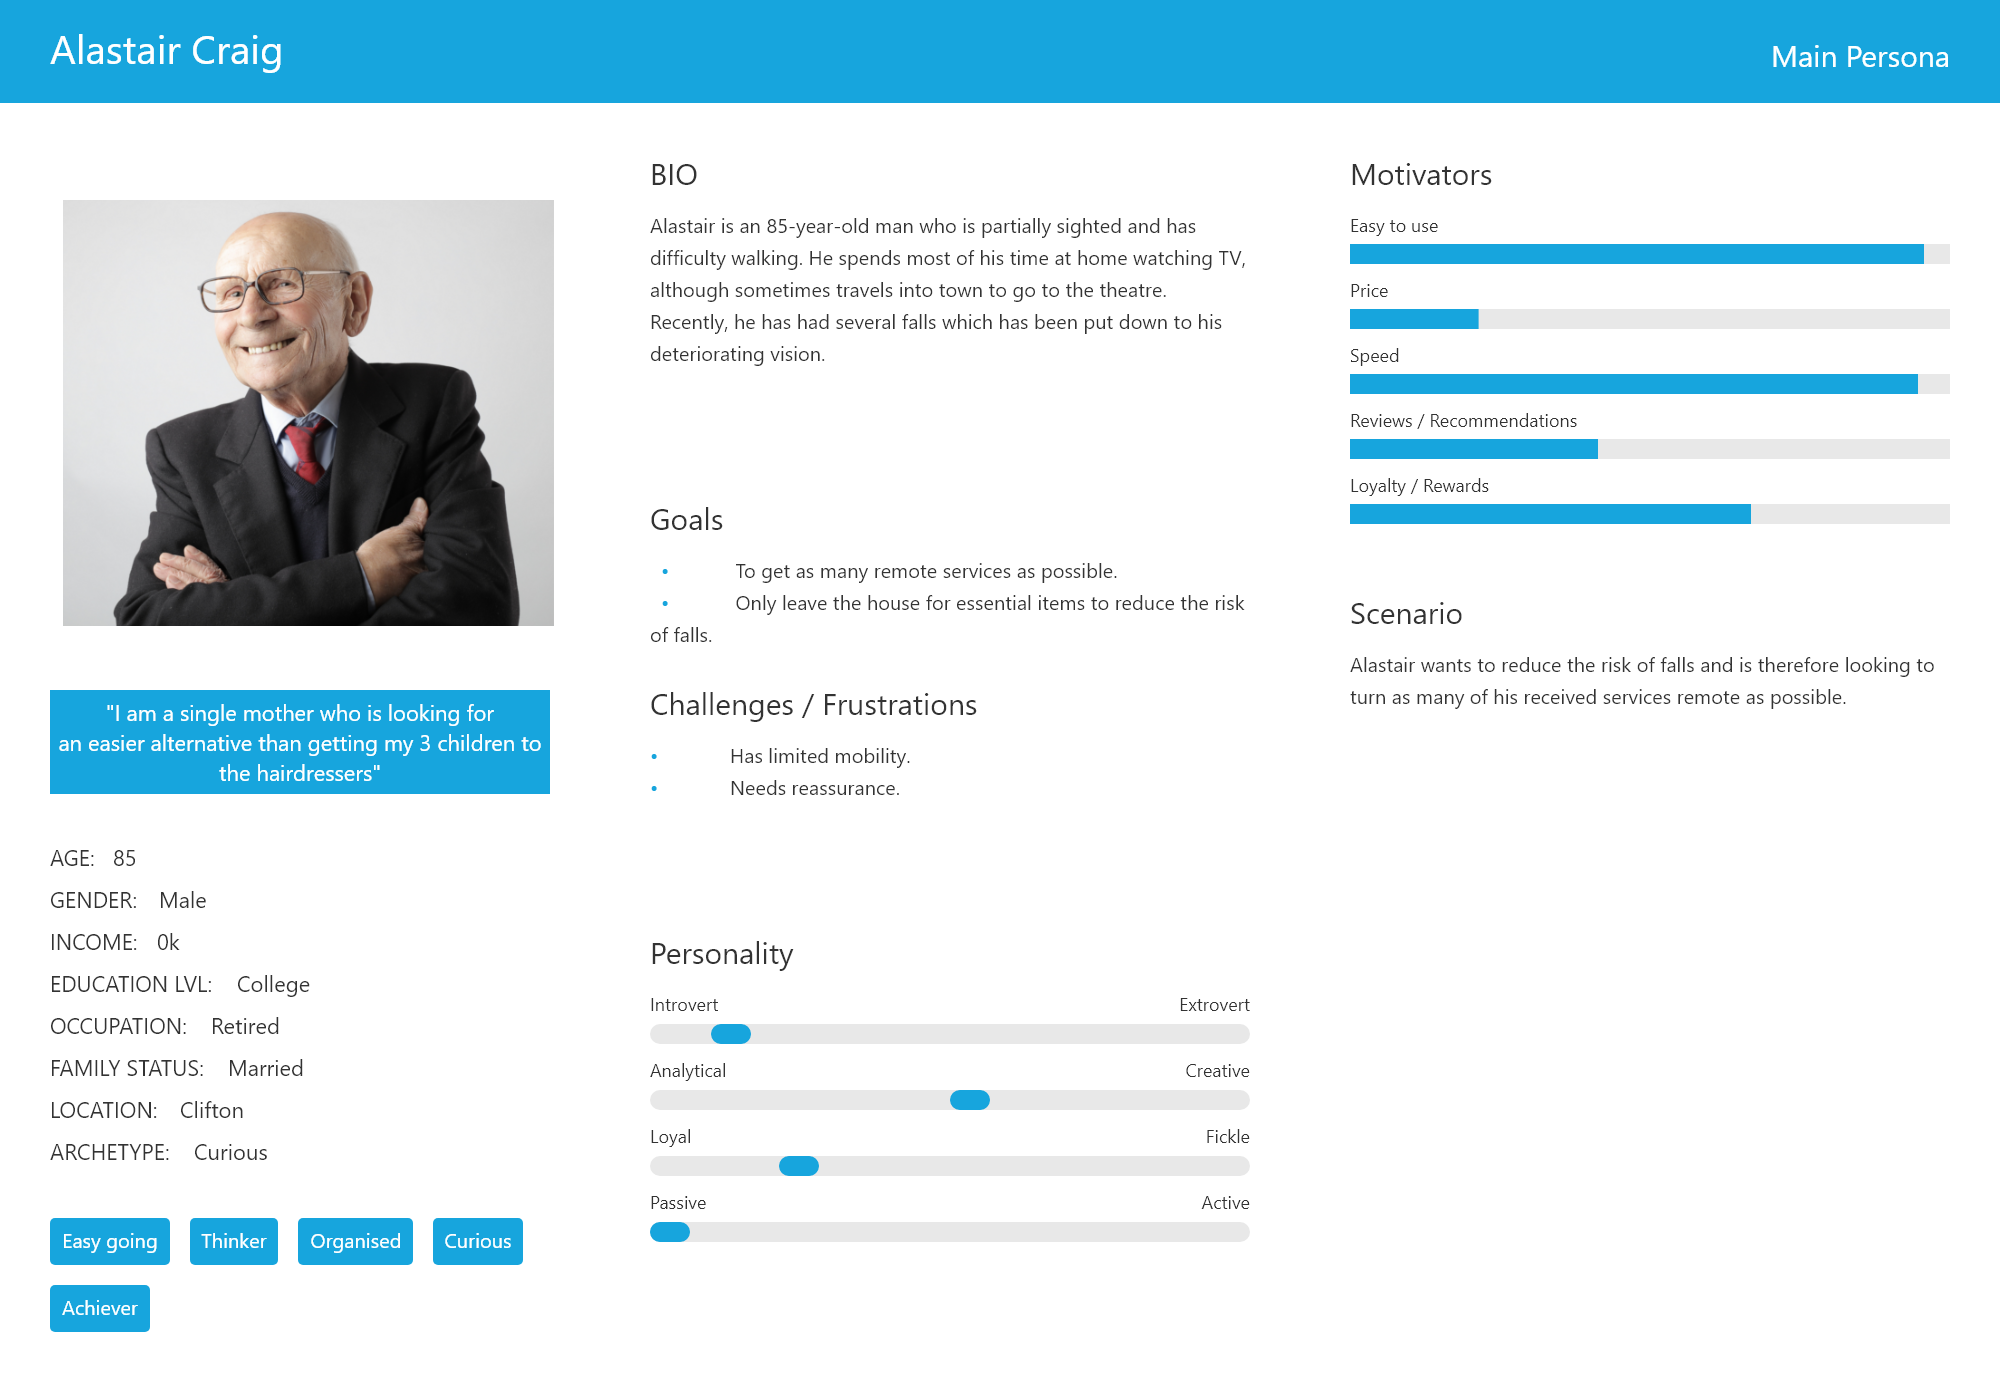
\includegraphics[scale=0.2]{images/persona_4.png}
			\caption{Persona 4}
			\label{fig:persona_4}
		\end{figure}
		
	\end{itemize}

	\section{Prototyping}
	An important component of UCD and more generally UX is wireframing, which involves making a mock-up of the application that acts as an early prototype to influence later development, along with allowing for early beta testing \cite{Arnowitz Arent Berger}. For the wireframing application Adobe XD was chosen for several reasons. Firstly, it has strong prototyping functionality, allowing the user to click around the application through the use of ‘components’. This interactivity means that early testers can get a real feel for how the application works. An illustration of this can be seen below, whereby each arrow represents a state change in the form of a trigger/ action pair, whereby for example a user could click on ‘Available Right Now’ and be taken to the ‘Checkout’ as seen in figure \ref{fig:prot-comp} below.
		\begin{figure}[H]
		\centering
		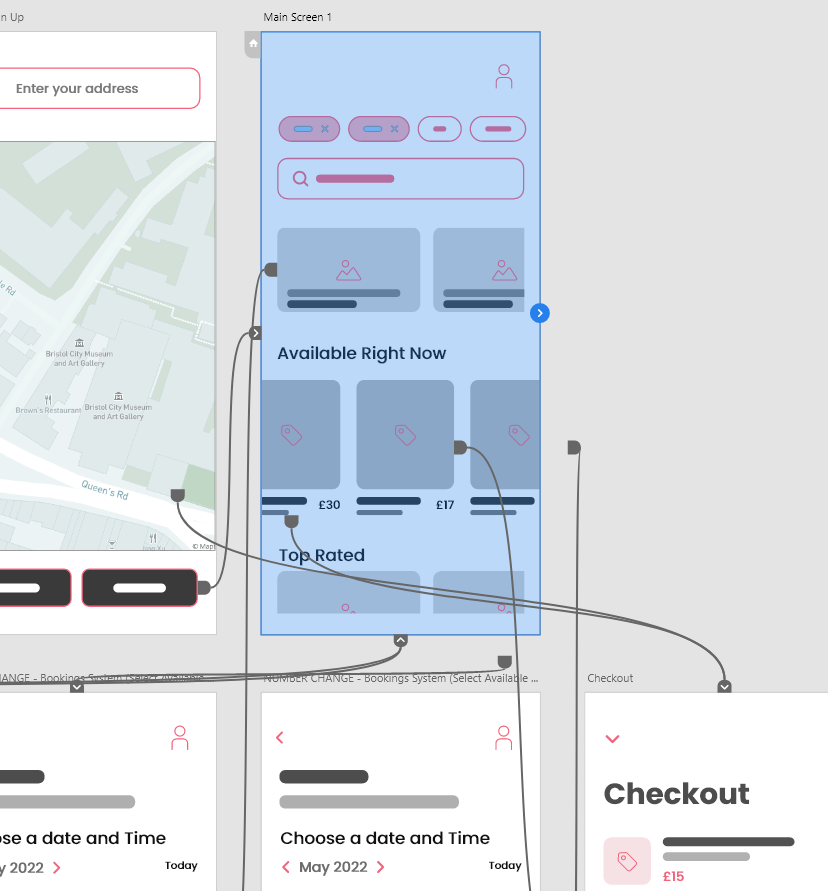
\includegraphics[scale=0.5]{images/prototyping-components.png}
		\caption{Component Interactivity within Adobe XD}
		\label{fig:prot-comp}
	\end{figure}
	
	
	Adobe XD also allows for easy distribution of the prototype in the form of a sharable link that opens in the browser and encompasses the same functionality and components that can be found within the application itself, meaning that anyone with access to a browser can test the prototype. Along with this, the prototype also allows for comments to be made, which are fed back to the owner. This comment capability was used early on during beta testing when it was sent out with the early questionnaire and influenced initial design decisions \cite{smashing-magazine}.
	
	When designing the screens there was a strong focus on user experience following Nielsons 10 Heuristics for User Interface Design \cite{nielson-normal-group-2020} . For example, the functionality was kept as minimal as possible to avoid clittering and avoid cognitive load on the user, the user was given control to go back and forward between previous screens to allow for user control and freedom and simple and self-explanatory language was used to apply recognition over recall. For example, the Sign In screen below extraneous text was kept to a minimum by using images for the login items, such as Google, Facebook and Twitter, a sign up button was included to allow the user to access the application through creating a new account and large, clear sign in forms and buttons were used. The full interactive Adobe XD wireframe can be found \href{https://xd.adobe.com/view/32f0c057-e909-40fa-b3d4-5610b0bda03c-67a3/}{here}. 
	
	\begin{figure}[H]
		\centering
		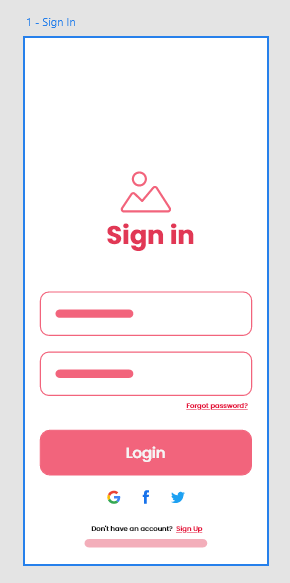
\includegraphics[scale=0.85]{images/sign-in.png}
		\caption{Sign In Page Made with Adobe XD}
		\label{fig:sign-in}
	\end{figure}
	
	\section{Production}
	\subsection{Version Control}

	
	\subsection{Sprint 1 - Setup}
	During the first sprint, the task involved setting up the environment in preparation to begin development. For the editor, Android Studio was 
	TALK ABOUT SCREENS/ MODELS/ HELPER etc
	\subsubsection{File Structure}
	Although there is no official recommendation for structuring the app, here we follow a commonly used structure which includes models; the files that serve as collections of data that are used in conjunction with the widgets to form the user interface of the application; providers; screens; utilities; and widgets; .

	
	
	\subsection{Sprint X - UI}
	Flutter offer an Adobe XD plugin to turn wireframes directly into code, however, this was not used for several reasons. In Adobe XD components are positioned absolutely, whereas in Flutter it is done relatively, leading to several issues with positioning. Adobe XD also does not contain customer properties and therefore mapping these to components, such as title is not possible.
	
	\subsubsection{Cupertino vs Material}
	The final project was built using material due to..
	
		\subsection{Sprint X - Login and Sign Up}
	Within the UserDatabase class, for the createNewUser function, we pass through the authentication uid, which is then used as the document id, so that future calls can refer to this and therefore fetch the document, without doing a call such as 
	\begin{lstlisting}
		_firebaseFirestore.collection(collection).where('uid', .isEqualTo('givenID')).get()
	\end{lstlisting}
	which does not scale well due to a search time of $\mathcal{O}$(n), compared to 
	\begin{lstlisting}
		_firebaseFirestore.collection(collection).doc(userId).get()
	\end{lstlisting}
	which gives a search time of $\mathcal{O}$(1). 	
	
	\subsection{Sprint X - Backend Design}
	
	Loading all parentBarbers/ barbers and products - 
	When entering the app it is more effecient to make one call to the server rather than multiple due to GPS restrictions. Therefore ParentBarbers, barbers and all of their products are loaded within a certain radius, rather than loading parentBarbers and barbers separately throughout the app. 
	
	Don't nest as calls will fetch all of the parent and nested structured so better to have separate data.
	
	\subsection{Sprint X - Location}
	https://firebase.google.com/docs/firestore/solutions/geoqueries
	Once the user logs in they give their location in the form of their address. This is stored in 'geohashes', which are longitude and latitiude co-ordinates that are hashed into a single Base32 string.
	
	User location access is granted through the following line in the ./android/app/src/main/AndroidManifest.xml file
	\begin{lstlisting}
		<uses-permission android:name="android.permission.ACCESS_FINE_LOCATION"/>
	\end{lstlisting}
	For the search results we use a drop down menu in the form of flutters built in 'showSearch' function loosely following a guide on medium \cite{medium-comerge} to display a search page and 'SearchDelegate' to define the content of said search page.
	
	A textEditingController is used to collect the inputted data from the user and pass through to the showSearch function.
	
	\subsubsection{Autocomplete locations}
	As a means for the user to autocomplete their address when signing up, the 'Place Autocomplete service', which returns location predictions in response to HTTP requests was implemented using a request adhering to a set of parameters, the full list, along with details of the API can be found on the Google Developers website \cite{requests}.
	First, we create a location model which can hold the data returned from the API. We then create an API request using the above aforementioned API format. For brevity, not every option is discussed, but those of importance include 'input', which is the user query, 'types', which determines the query returned, for which we specify address to return the full address and 'sessionToken', which is required for each new query. The query can be seen here:
	\begin{lstlisting}
		'https://maps.googleapis.com/maps/api/place/autocomplete/json?input=$input&types=address&components=country:ch&lang=en&key=$apiKey&sessiontoken=$sessionToken';
	\end{lstlisting}
	The returned results are in json format and after some minor error checking we parse using json.decode into a list with our LocationModel class, whilst assigning a new UUID for each query (Google recommends to use version 4 UUID and so this is used here). Without our 'user\_gps.dart' file
	
	For the content of the search page we use pass in newly created session token into the ShowSearchPage class, which in turn sends an api request and parses the json data to return a list of locations in the form of 'place id's' and 'description' using a FutureBuilder. From here, we pass through the location id to the getLocationDetails function to fetch the address details of each location and then display this to the user.
	
	\subsection{Widgets and Common Items}
	Here we discuss any items not covered within a specified sprint.
	
	\subsubsection{Widgets}
	Several widgets were used to increase readability and brevity of code. For example, 'return\_text.dart' allows for access to the main components of the Text function and 'return\_image.dart' allows for easy use of the NetworkImage function, giving brevity and readability to the code.
	
	\subsubsection{Common Items}
	The common items contains global variables that were accessible throughout the project. Initially this included structures and arrays that served as objects to test the functionality of the frontend, for example a barber shop class with a nested list of barbers classes, each with a name, age, description etc. As backend functionality was added these items were removed. A theme class was then added which contains dart files that can be implemented. Doing it in this way meant that the application could be easily styled, without any unnecessary refactoring of code.
	
	

	
\end{document}